\documentclass{article}
\usepackage[utf8]{inputenc}

\usepackage{pseudocode}
\usepackage{multirow}
\usepackage[hidelinks]{hyperref}
\usepackage{indentfirst}


\usepackage{lettrine}
\usepackage{lipsum}
\usepackage{Zallman} % font
\usepackage{color}
\usepackage{listings}

\usepackage{graphicx}
\graphicspath{ {.} }

\renewcommand{\LettrineFontHook}{\Zallmanfamily}
\renewcommand{\LettrineTextFont}{\Huge\scshape}

\title{Reinforcement Learning vs Genetic Algorithm Optimization for Robot Walking}
\author{Noah Driker, Jason Tran, Luke Ren, Farbod Ghiasi}
\date{December 2021}

\begin{document}

\maketitle

\section{Problem Statement}
\lettrine[lines=5]{T}{he}
     goal of this project is to compare the quantitative results of the 
performance of reinforcement learning and genetic algorithm optimization 
techniques on the problem of teaching a robot to walk. The performance of the
robot walking will be simulated using the MuJoCo physics \cite{mujoco} engine
library. These methods will be used to maximize the reward function defined 
by the MuJoCo physics engine library, which rewards the robot for walking 
farther distances, with the constraints defined by the MuJoCo physics engine.

\section{Previous Work}

    In order to evaluate the performance of both a reinforcement learning 
algorithm and genetic algorithm, research was conducted on both fields of 
algorithms in order to determine the optimal implementations to test and 
compare with. However, these algorithms required a simulated environment, 
ideally one based on physical constraints, to be tested on. After conducting 
research on various physics engines, it was decided that MuJoCo, the 3D 
physics environment developed by OpenAI as a part of the OpenAI Gym 
\cite{openaigym} toolkit, would be used to compare the  performance of the 
different algorithms. The MuJoCo physics engine defined the constraints on 
the input variables of the optimization problem, as well as the reward 
function whose value would be maximized as the 
overarching optimization problem. With the physics environment decided and 
optimization problem defined, it was required to look into the optimal 
approach for the reinforcement learning algorithm and genetic algorithm.
    
    The approach to reinforcement learning that was taken to maximize the 
distance travelled by the robots defined in MuJoCo was Proximal Policy 
Optimization. The different forms of this algorithm are described in the 
paper, \emph{Proximal Policy Optimization Algorithms} by John 
Schulman, Filip Wolski, Prafulla Dhariwal, Alec Radford, and Oleg Klimov \cite{ppo}. The
paper details the algorithm's use of a clipped surrogate objective function 
and an adaptive penalty coefficient to obtain strong performance on 
continuous domain optimization problems. This algorithm was chosen because 
the environments provided by MuJoCo were continuous domain environments, and 
there were many available implementations and resources to use as a 
foundation for our implementation. For this project, an implementation for 
PPO from the open-source library, RLlib \cite{rllib}, was integrated and 
tuned to maximize the reward function defined  in the MuJoCo physics 
environment according the the constraints defined. Likewise, a similar 
approach to deciding the genetic algorithm was taken.

    The genetic algorithm that was implemented in this project was written 
without a predefined library or framework, but took influence from the book, 
\emph{Algorithms for Optimization} \cite{algorithmsforoptimization} by  Mykel
J. Kochenderfer and Tim A. Wheeler, which defined four phases: 1- Initial Population, 
2- Selection, 3- Crossover, and 4- Mutation. A predefined framework was not used in order to give
the genetic algorithm the most flexibility in terms of configuration and 
design. Because the algorithm was not extracted from a third-party library, we were able to make alterations and tune it
to the specifics MuJoCo environments, as well as
include custom population reduction and selection methods. In order to 
improve the performance of the genetic algorithm, a version of the algorithm 
applied a technique similar to gradient accelerating momentum, and acted as a feedback control loop for the convergence parameters. This momentum allowed the  
algorithm to widen its search for the optimum, and also allowed it to more easily find minima by introducing a 
momentum factor that decays over time to prevent overshooting. With the 
background of these algorithms laid out, the project was then divided into 
portions for each group member to work on.

\section{Decomposition}
    
    The project was divided into three portions, split among the group members  
Noah Driker, Farbod Ghiasi, Luke Ren, and Jason Tran \cite{authors}. Jason 
Tran  worked on integrating the PPO algorithm defined in the open-source 
library,  RLlib, with the physics environments defined in MuJoCo, which 
included defining an objective function and logging quantitative metrics. Logging and tuning for the reinforcement learning algorithm was also performed using NXDO \cite{nxdo}.
Noah Driker and Farbod Ghiasi worked on designing and tuning the custom genetic 
algorithm to optimize the same environments in MuJoCo. Luke Ren worked on 
writing and preparing the report, as well as organizing meetings and 
synthesizing discussions on the implementations of the algorithms. The Python 
packages, gym and mujoco-py, contained all of the definitions for the physics environments used to test the optimization methods, which were developed by  
OpenAI. The Python package, ray, contained the code for the open-source 
library RLlib, used to implement the proximal policy optimization algorithm. Logging and graphing was performed using the matplotlib \cite{matplotlib} and tensorboard packages.

The project began with the whole team conducting research on possible 
Reinforcement Learning and Genetic Algorithms to compare, which resulted in 
the use of PPO for Reinforcement Learning and a natural selection based 
algorithm for the genetic algorithm. Jason Tran, then, developed the program 
to apply RLlib for PPO on the MuJoCo project, which also included generating    plots for performance statistics on the algorithm. Noah Driker and Farbod     Ghiasi designed and developed the genetic algorithm, which involved deciding
a population reduction heuristic and a population selection decision. They, 
then, applied the algorithm to the MuJoCo physics environments and measured 
the same performance statistics as for the reinforcement learning algorithm.
Luke Ren prepared the report, including outlining the problem statement, 
previous work, and analyzing the results in the paper, as well as the poster.


\section{Coding Work}
\noindent\textbf{Genetic Algorithm}



The Genetic Algorithm, inspired by biological evolution, uses an iterative process to produce fitter candidates (aka cands). The process begins by initializing the genesis, a population of randomly generated candidates that will begin the search towards the optimum. Every candidate for this simulation is an action, i.e. an ordered sequence of moves that is fed to the physics environment to control the agent. The algorithm, at every iteration, evaluates every candidate in the generation for fitness, and stores the result (reward). Then, at the end of the evaluation period for each generation, the population is sorted in increasing order of fitness, and the algorithm removes the unfit candidates; this mimics the process of natural selection in biological evolution. The number of candidates that perish is decided by a hyperparameter (see Decimal Perish in the table below). Following the selection of candidates, the algorithm augments the population to include more of the fitter candidates. This is done to increase the likelihood that the fitter candidates will mate. Finally, candidates are mated together randomly, until the number of new candidates equals the next generation size, a parameter that is controlled by a few update functions described below.

Our group made a few modifications to the Genetic Algorithm to improve the rate of learning and to increase the max achieved reward. These include adaptive mutation rates and an oscillating next generation size. There are two functions in our genetic algorithm implementation that are responsible for these adjusting parameters: updateParamsAfterGen() and updateAfterStagnation(). The updateParamsAfterGen() function is called after every generation, and gradually decreases the mutation rate and next generation size to urge the algorithm towards convergence. The updateAfterStagnation() function is called after the maximum achieved reward has stayed the same for 3 or more iterations. Since the agent has not improved for multiple consecutive iterations, the function increases the Mutation Rate and the Next Generation Size to attempt at leaving the local minimum. Mutation Rate is increased to introduce possibly new genes into the pool, and Next Generation Size is increased to promote higher genetic diversity among the offspring. These functions work together to create a feedback control loop, as they automatically adjust the convergence parameters for the simulation.

Lastly, we entered the best candidate of the current generation into the next population, to guarantee that the best candidate among all, is present in the final generation.

In the table below, we listed the hyperparameters used to control the simulation, and the values that we chose to use.\\


\begin{tabular}{ |p{3cm}|p{6cm}|p{1cm}|  }
 \hline
 \multicolumn{3}{|c|}{Hyperparameters} \\
 \hline
 Parameter & Description & Value\\
 \hline
 Action Len   & Number of moves per action & 1000\\
 First Gen Size &   Number of candidates in first gen  & 1000\\
 Default Next Gen Size  &  Maximum Next Gen Size & 500\\
 Num Generations&   Length of simulation in generations  & 2000\\
 Decimal Perish & Decimal part of population that will perish  & 0.6\\
 Default Chance of Mutation & Initial Chance of Mutation  & 0.25\\
 \hline

\end{tabular}\\

The Action Length was chosen to be 1000, as this is the maximum number of moves that the agent can perform in the environment before it is reset. We chose a large number for the First Generation Size (1000), in order to increase genetic diversity in the initial population, and to increase the probability of starting our search in the right direction. The Default Next Generation Size was chosen to be 500, because our algorithm needs enough room for growth when it becomes stagnant. We chose Number of Generations to be 2000, although we've never ran our algorithm with this many generations; the algorithm usually achieves its maximum before this, and is no longer able to improve. The Decimal Perish parameter is selected to be 0.6 (meaning 60\% of the population will perish). This was chosen in order to remove the majority of poor performers, but also to keep enough of the population to promote genetic growth. Finally, the Default Chance of Mutation was chosen to be 0.25. This initially forces the mutation rate to be high, so that the algorithm is able to explore many different possible candidates, but the mutation rate is decreased at each iteration with the updateParamsAfterGen() function, to allow the algorithm to converge. 

Below are some of the essential pieces used in our implementation of the Genetic Algorithm.


        



\begin{pseudocode}[shadowbox]{PerformNaturalSelection}{Population} 
\\\COMMENT{ Remove unfit cands, create next set of parents}\\

\\ numPerish\GETS percentPerish * len(Population)
\\ sorted\GETS sort(Population)
\\ pruned\GETS sorted[numPerish: End]

\\ nextParents\GETS [ ]\\
\\\COMMENT{ Increase the likelihood of more fit candidates mating}\\

\FOR i\GETS 0 \TO len(pruned) \DO
    \BEGIN 
        \FOR j\GETS 0 \TO i + 1 \DO
                nextParents.\CALL{add}{pruned[i]}\\ 

    \END\\
\RETURN{nextParents}

\end{pseudocode}
% ======== Algorithm 4.1 start ================
\\
Algorithm 4.1. performs mimics natural selection by removing the poor performing candidates from the population. This Algorithm takes a Population, sorts it in order of increasing candidate reward, and returns the pruned population. This pruned population will be the parents of the next generation.

% ======== Algorithm 4.1 end ================


\begin{pseudocode}[shadowbox]{Crossover}{Parent1, Parent2, p1First} 
\COMMENT{See code for implementation}\\
\COMMENT{If p1First, Parent1 contributes to first half of genome}\\
\RETURN{combinedGenome}

\end{pseudocode}
% ======== Algorithm 4.2 start ================ NEEDS WORK
\\
Algorithm 4.2. implements genetic crossover. The third parameter, p1First, is the result of a coin-flip done in Algorithm 4.3. This coin-flip decides which Parent will contribute the first half of their genome to the offspring. This algorithm achieves genetic crossover by combining the first half of one parent's genome with the second half of the other parent's genome. 
% ======== Algorithm 4.2 end ================


\begin{pseudocode}[shadowbox]{Mate}{Parent1, Parent2} 
\COMMENT{Crossover and Mutate}\\
parent1First = \CALL{RandomChoice}{True, False}\\

newGenome\GETS \CALL{Crossover}{Parent1, Parent2, parent1First}\\
geneIndex\GETS 0\\
\FOREACH gene \in \mathcal{} newGenome \DO
\BEGIN
    \IF (\CALL{RandomBetween}{0, 1} <= chanceOfMutation) \THEN \BEGIN
        newGene\GETS \CALL{CreateRandomGene}{}\\
        newGenome.\CALL{replace}{gene, newGene}
        
    \END
    
\END\\
\RETURN{newGenome}

\end{pseudocode}
% ======== Algorithm 4.3 start ================ NEEDS WORK
\\
Algorithm 4.3. implements mating among candidates. Mating involves performing genetic crossover with the two given parents, and deciding by chance whether to mutate a gene in the genome. This algorithm returns the new genome.

% ======== Algorithm 4.3 end ================

\begin{pseudocode}[shadowbox]{MateParents}{Parents} 
\COMMENT{Randomly mate parents to create next generation}\\
nextGeneration\GETS [ ]
\\ candidatesCreated\GETS 0\\
\WHILE candidatesCreated < nextGenerationSize \DO
    \BEGIN
    p1, p2\GETS \CALL{RandomlySelectTwo}{Parents}\\
    newCandidate\GETS \CALL{Mate}{p1, p2}\\
    nextGeneration.\CALL{add}{newCandidate}\\
    candidatesGenerated \mathrel{+}= 1\\
    \END\\
\RETURN{nextGeneration}

\end{pseudocode}
% ======== Algorithm 4.4 start ================
\\
Algorithm 4.4. randomly selects pairs of parents to mate, and returns the next generation of candidates.

% ======== Algorithm 4.4 end ================

\begin{pseudocode}[shadowbox]{CreateNewGeneration}{Population} 
    newParents\GETS \CALL{PerformNaturalSelection}{Population}\\
    nextGeneration\GETS \CALL{MateParents}{newParents}\\
    \RETURN{nextGeneration}
\end{pseudocode}
% ======== Algorithm 4.5 start ================
\\
Algorithm 4.5. uses Algorithm 4.1 and Algorithm 4.4 to create a new generation from the current population.

% ======== Algorithm 4.5 end ================

\begin{pseudocode}[shadowbox]{evolve}{ } 

generationIndex\GETS 0\\
\WHILE (generationIndex  < numGenerations) \DO
\BEGIN
    population\GETS \CALL{GenerateGenesis}{}\\
    \FOREACH candidate \in \mathcal{} population \DO
    \BEGIN
        candidate.reward = \CALL{EvaluateCandidate}{}\\
    \END\\
    population = \CALL{CreateNewGeneration}{population}\\
    \CALL{UpdateParameters}{}\\
    \CALL{UpdateAfterStagnation}{}\\
    
\END\\


\end{pseudocode}
% ======== Algorithm 4.6 start ================
\\
Algorithm 4.6. implements the core of the Genetic Algorithm. Evolve generates the genesis, and iteratively steps through each generation, evaluating each candidate, creates new generations, and updates the convergence parameters.
\\

% ======== Algorithm 4.6 end ================



\noindent\textbf{Reinforcement Learning}

    Reinforcement Learning is a form of machine learning that trains an agent to learn and perform tasks in an environment with a reward and observation in mind. For this project we have an agent learning to either walk as a Half Cheetah or as a Humanoid inside of the MuJoCo environment. In order for an agent to learn, it needs a policy\footnote{An approach or strategy an agent utilizes to accomplish a task.} which maximizes the reward obtained for an action. To do so, policy gradient methods are often used to optimize policies with respect to the reward it generates by using gradient descent. Proximal Policy Optimization (PPO), a simpler and more effective variant of Trust Region Policy Optimization (TRPO)\footnote{Another policy gradient method often used in reinforcement learning which uses trust regions to optimize policies.}, is used in this project to train an agent to walk in different MuJoCo environments. The implementation of PPO used to train agents is from Ray RLlib\footnote{An open source library for reinforcement learning.} in Python.
    \newline
    \indent A baseline of the reinforcement learning section of the project was initially created to ensure that the MuJoCo OpenAI environment worked. The agent of this version only had random actions and did not learn. Afterwards, a basic implementation using Ray RLlib was created and tested. The reward per iteration of the this version was logged into a text file and graphed via python's matplotlib library as it was simply to test if the agent was learning. The last and final implementation used a different logger and simplified the environment class. This version viewed graphs through tensorboard and its hyperparameters were tuned via the Ray tune library in-order to optimize the trainer for better rewards. The logger and tuning implementation used for the final reinforcement learning version are from nxdo\cite{nxdo}.

\section{Quantitative Results}

The results for the performance of the genetic algorithm on the Half Cheetah environment in MuJoCo are given in \autoref{fig:gaHalfCheetahResults}.
The results for the performance of the genetic algorithm on the Humanoid environment are given in \autoref{fig:gaHumanoid}.

\begin{figure}
    \centerline{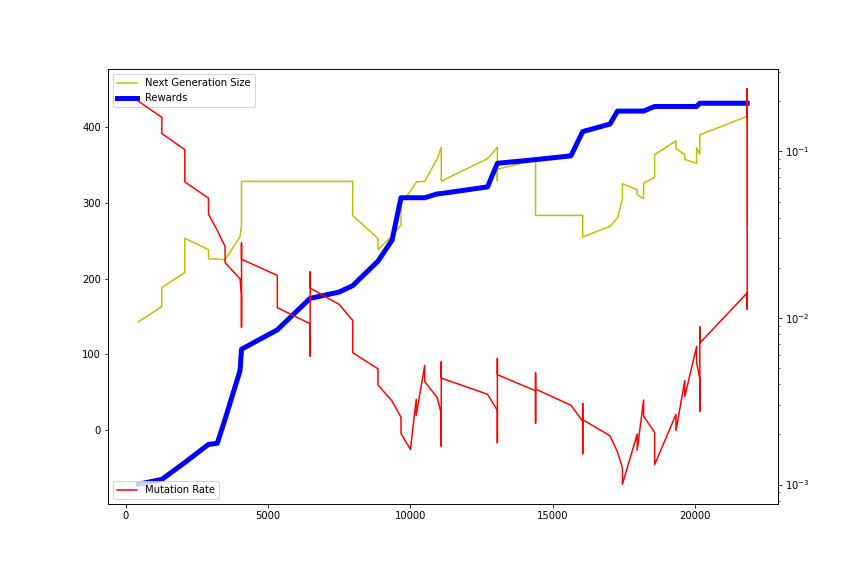
\includegraphics[scale=0.5]{tripleGraph_hc.png}}
    \caption{Reward, Mutation Rate, and Next-Generation Size for Half Cheetah}
    \label{fig:gaHalfCheetahResults}
\end{figure}

\begin{figure}
    \centerline{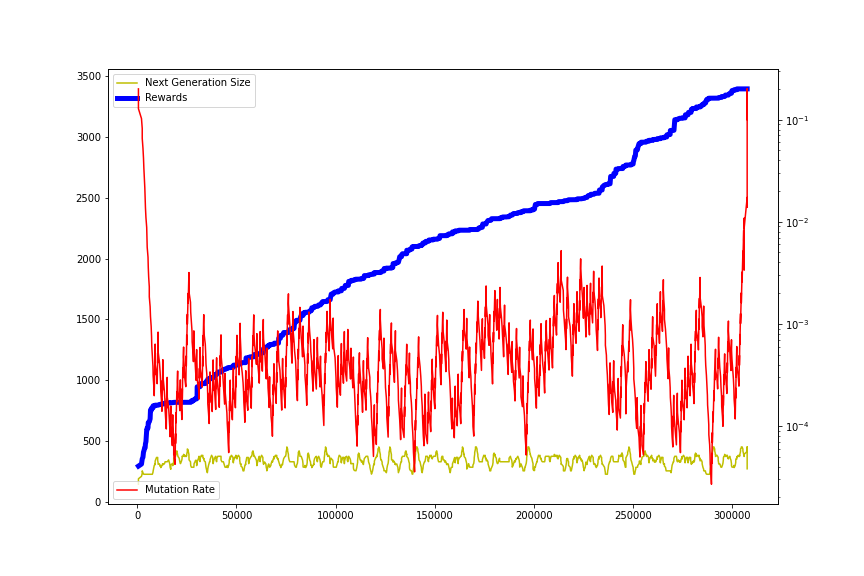
\includegraphics[scale=0.5]{tripleGraph_human.png}}        
    \caption{Reward, Mutation Rate, and Next-Generation Size for Humanoid}
    \label{fig:gaHumanoid}
\end{figure}

    In the performance graphs, the total rewards yielded at each iteration of the algorithm are graphed against both the mutation rate and next generation size values, which are also adapted at each iteration. For both environments after 15 hours of training, the total rewards value has a strong positive correlation with the number of iterations, but the performance improved more slowly over time, with the total maximum reward reaching around 3300 for the Humanoid environment and 450 for the Half Cheetah environment. For the Half Cheetah graph, the next generation size maintains a weak positive correlation with the number of iterations, identifying that the algorithm is slowly increasing the generation size as the number of iterations increases. This correlation is less clear for the Humanoid graph, but the positive correlation is still identifiable. This correlation can be attributed to the population allowing a larger search space for the algorithm to improve. The sharp increases in mutation rate are also correlated with improvements in the total rewards value, which can be attributed to the mutation rate diversifying the search space of the algorithm, with the reduction of the mutation rate allowing the individual models to converge towards local minima.
    
\begin{figure}
    \centerline{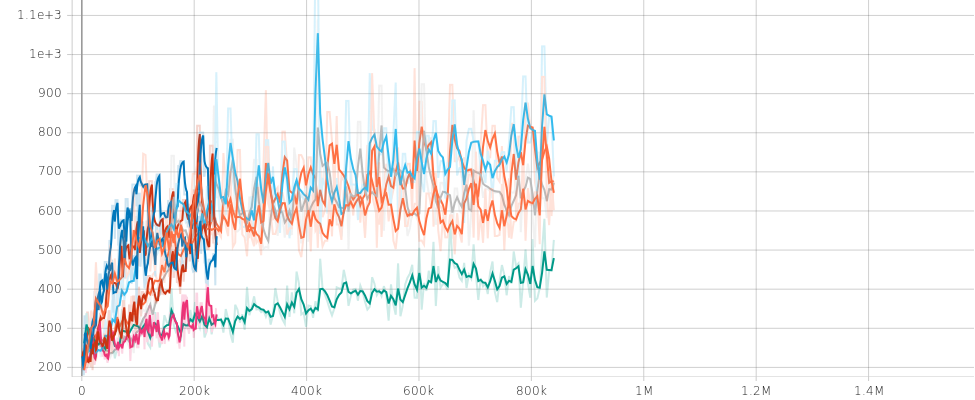
\includegraphics[scale=0.5]{humanoid_tuner_reward_max.png}}        
    \caption{Max Episode Reward Tuning Result for Humanoid}
    \label{fig:rlHumanoid}
\end{figure}
\begin{figure}
    \centerline{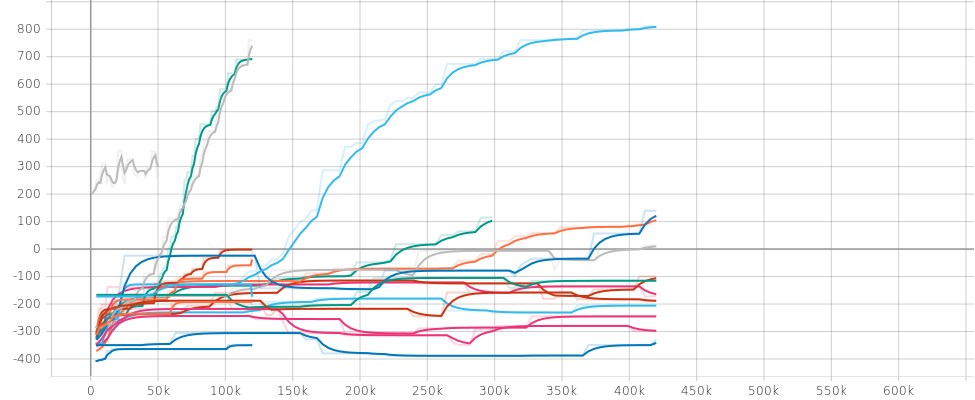
\includegraphics[scale=0.5]{halfcheetah_tune_episode_reward_max.png}}        
    \caption{Max Episode Reward Tuning Result for Half Cheetah}
    \label{fig:rlHalfCheetah}
\end{figure}

    In \autoref{fig:rlHumanoid} and \autoref{fig:rlHalfCheetah}, the results of parameter tuning the reinforcement learning algorithm, Proximal Policy Optimization, on the Humanoid and Half Cheetah physics environments from MuJoCo are displayed respectively. The different lines represent different combinations of hyper parameter values chosen when tuning the algorithm. By performing tuning, the best combination of hyper parameters from the sample can be decided before training with the algorithm over an extended period of time.
    
\begin{figure}
    \centerline{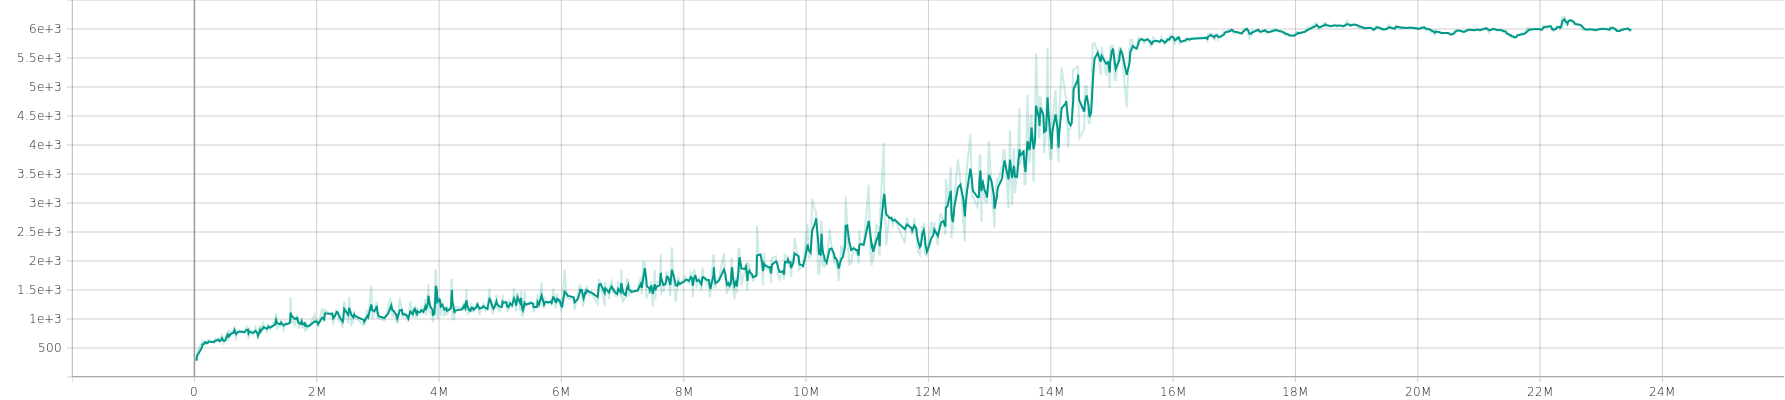
\includegraphics[scale=0.3]{best_humanoid.png}}        
    \caption{Training Results for Humanoid (Reinforcement Learning)}
    \label{fig:rlHumanoidRes}
\end{figure}
\begin{figure}
    \centerline{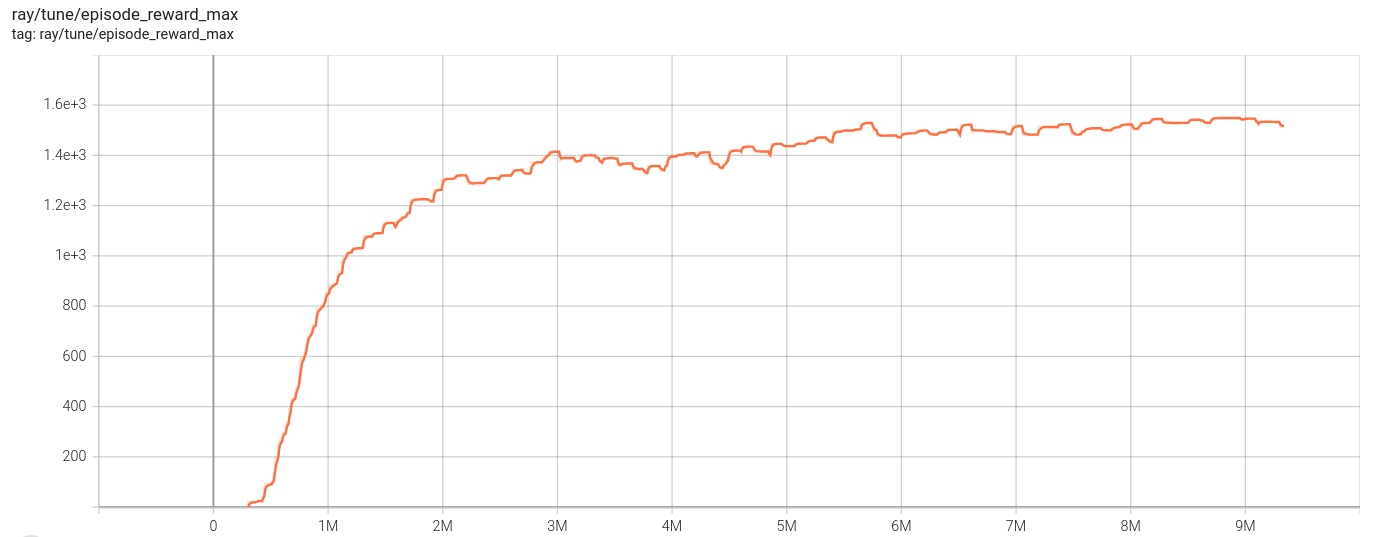
\includegraphics[scale=0.3]{best_halfcheetah.png}}        
    \caption{Training Results for Half Cheetah (Reinforcement Learning)}
    \label{fig:rlHalfCheetahRes}
\end{figure}
    The performance graphs for reinforcement learning when trained on the Humanoid environment are displayed in \autoref{fig:rlHumanoidRes} and \autoref{fig:rlHalfCheetahRes} respectively. The graphs identify a strong positive correlation between the total rewards and number of iterations ran for the algorithm, however, the performance seems to taper off for the Humanoid environment around the 15 million iteration mark and the Half Cheetah environment around the 3 million iteration mark. Although the algorithm was run for 8 hours for both environments, the algorithm stopped improving significantly around the 6 hour mark for the Humanoid environment and around the 4 hour mark for the Half Cheetah environment. Given this amount of time, the algorithm was able to achieve a maximum total reward value of around 6,000 for the Humanoid environment and 1,500 for the Half Cheetah environment.
    
    Comparing the performance of the two algorithms, although reinforcement learning required a tuning phase to decide the best parameters, the overall training time and maximum rewards were better for reinforcement learning. For the Humanoid environment, the reinforcement learning algorithm was able to achieve a total maximum reward of over 6,000 after 8 total hours of training, while the genetic algorithm achieved a total maximum of around 3,500 after 15 hours of training. For the Half Cheetah environment, the reinforcement learning algorithm was able to achieve a total maximum reward of over 1,500 after 8 total hours of training, while the genetic algorithm achieved a total maximum reward of around 450 after 15 total hours of training.
    
    
\section{Conclusion}
    Based on the results mentioned above, as well as a visual analysis of the graphs produced by training with both optimization algorithms on the MuJoCo physics engine environment, it can be concluded that the reinforcement learning algorithm had a stronger overall performance. While both algorithms yielded strong positive correlations for the reward over the number of iterations, the reinforcement learning algorithm implemented using PPO was able to yield higher total maximum rewards quicker. Thus, it can be concluded, given the amount of time and processing power available, that the reinforcement learning algorithm has overall better performance than the genetic algorithm for the continuous, constrained optimization problem of maximizing reward in a simulated robot walking environment.
    
\section{Possible Improvements}
    Although the Genetic Algorithm and Reinforcement Learning were able to simulate a half cheetah and humanoid walking, they can still attain superior rewards to what was presented in this report. Genetic Algorithm can be improved by using a feedback control algorithm, such as AIMD\footnote{Additive Increase/Multiplicative Decrease} or MIAD\footnote{Multiplicative Increase/Additive Decrease}, to better control the mutation rate and next generation size. Furthermore, Genetic Algorithm could be implemented differently in a manner similar to NEAT\footnote{NeuroEvolution of Augmenting Topologies} which is an evolutionary algorithm that creates artificial neural networks\cite{neat}. As for Reinforcement Learning, allowing more time and access to additional computational power would greatly improve the results. When tuning the hyperparameters for Reinforcement Learning, the time allotted for tuning did not exceed 8 hours and only 4-8 cores were allowed and no GPUs were used for further computational power. Allowing for more time would allow the tuner to find more hyperparameters to test while more computational power would allow testing to occur much faster. As a result, the tuner would be able to optimize the hyperparamters much faster and efficiently. 
    
%Sets the bibliography style to UNSRT and imports the 
%bibliography file "references.bib".
\bibliographystyle{unsrt}
\bibliography{references}


\end{document}
